% Created 2020-09-29 Tue 15:39
% Intended LaTeX compiler: pdflatex
\documentclass[presentation]{beamer}
\usepackage[utf8]{inputenc}
\usepackage[T1]{fontenc}
\usepackage{graphicx}
\usepackage{grffile}
\usepackage{longtable}
\usepackage{wrapfig}
\usepackage{rotating}
\usepackage[normalem]{ulem}
\usepackage{amsmath}
\usepackage{textcomp}
\usepackage{amssymb}
\usepackage{capt-of}
\usepackage{hyperref}
\usetheme{UoB}
\author{Mark Blyth}
\date{\textit{[2020-09-30 Wed]}}
\title{Deterministic continuation of stochastic metastable equilibria via Lyapunov equations and ellipsoids}
\hypersetup{
 pdfauthor={Mark Blyth},
 pdftitle={Deterministic continuation of stochastic metastable equilibria via Lyapunov equations and ellipsoids},
 pdfkeywords={},
 pdfsubject={},
 pdfcreator={Emacs 27.1 (Org mode 9.3)}, 
 pdflang={English}}
\begin{document}

\maketitle

\section{Background / intro}
\label{sec:org68ea7ef}
\begin{frame}[label={sec:org68b1949}]{Background}
\begin{itemize}
\item Numerical continuation is a useful tool for deterministic systems
\end{itemize}
\vfill
\begin{itemize}
\item Stochastic dynamics can't be studied with standard continuation
\end{itemize}
\vfill
\begin{itemize}
\item This work tries to change that
\end{itemize}
\end{frame}

\section{Section 1}
\label{sec:org8791e91}
\begin{frame}[label={sec:orgd74b88a}]{Section 1: Intro}
Deterministic systems:
\vfill
\begin{itemize}
\item Equilibrium = time-invariant solution
\end{itemize}
\vfill
\begin{itemize}
\item Equilibrium state depends on parameters
\end{itemize}
\vfill
\begin{itemize}
\item Continuation reveals that dependence
\end{itemize}
\end{frame}

\begin{frame}[label={sec:org29e5707}]{From deterministic to stochastic}
\begin{itemize}
\item Very little work to extend continuation to SDEs
\end{itemize}
\vfill
\begin{itemize}
\item How does small noise change deterministic results?
\end{itemize}
\vfill
\begin{itemize}
\item We can extend numerical continuation to track local information about metastable equilibria
\end{itemize}
\end{frame}

\section{Section 2}
\label{sec:org1f5331a}
\begin{frame}[label={sec:org909b779},plain]{An analytical example}
Consider a noise-corrupted pitchfork normal form

\begin{center}
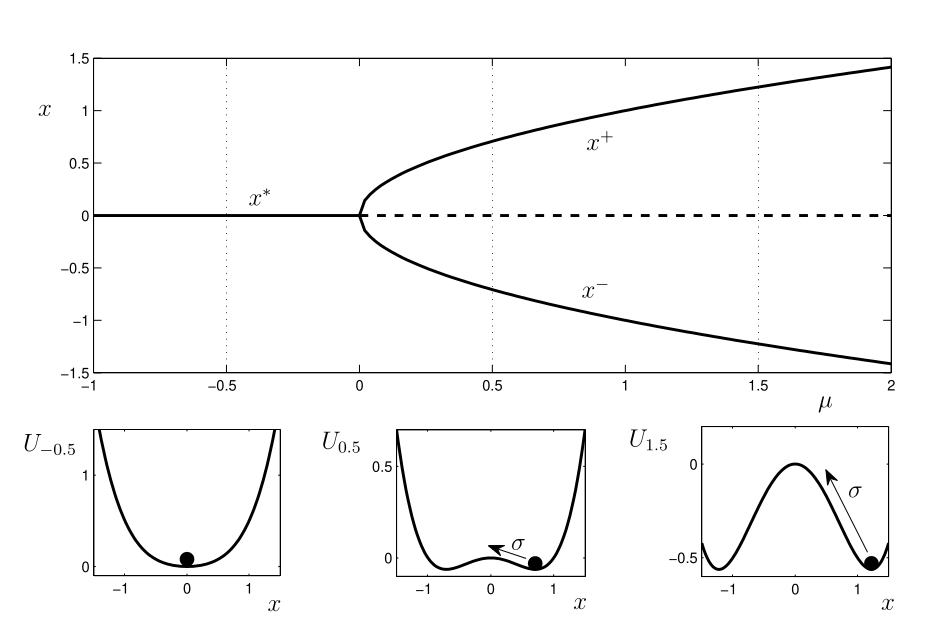
\includegraphics[width=.9\linewidth]{./pitchfork.png}
\end{center}
\end{frame}

\begin{frame}[label={sec:orgcf9bbc8}]{Noise-induced pitchfork dynamics}
\begin{itemize}
\item Interesting noise-induced dynamics occur in the bistable region
\end{itemize}
\vfill
\begin{itemize}
\item For any initial condition, we will almost surely visit visit both potential wells in finite time
\end{itemize}
\vfill
\begin{itemize}
\item We seek a stronger result; what insights can we gain into the timescales of the stochastic transitions?
\end{itemize}
\end{frame}

\begin{frame}[label={sec:orgfd0236c}]{A graphic example}
\begin{center}
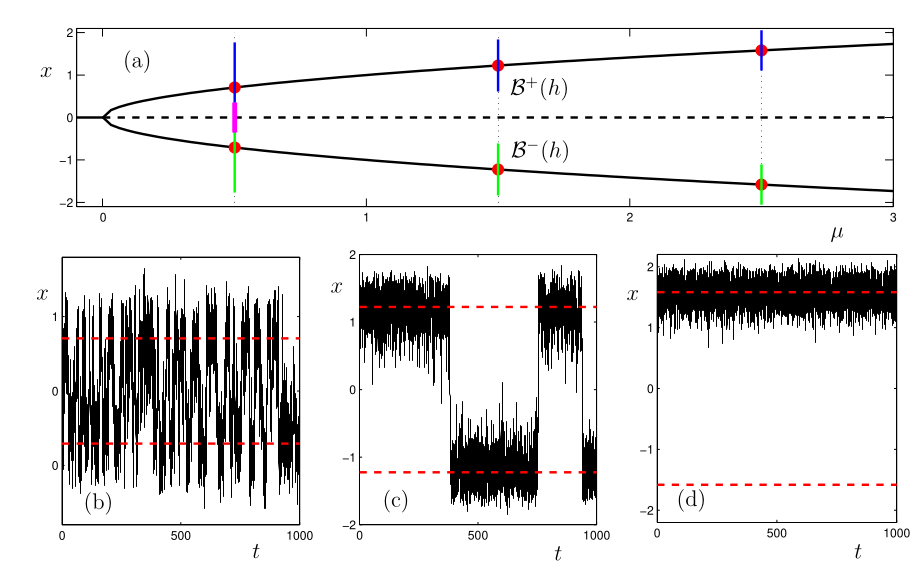
\includegraphics[width=.9\linewidth]{./neighbourhoods.png}
\end{center}
\end{frame}
\begin{frame}[label={sec:org3246785}]{Studying stochastic transitions}
\begin{itemize}
\item What methods can we use to study the high-density regions?
\end{itemize}
\vfill
\begin{itemize}
\item Fokker-Planck equations are inefficient
\end{itemize}
\vfill
\begin{itemize}
\item Can we find a more efficient way of defining them?
\end{itemize}
\end{frame}

\begin{frame}[label={sec:org7b265a4}]{Continuation of metastable equilibria}
Can we find a more efficient way of defining high-density regions?
\vfill
\begin{itemize}
\item Linearise the system about each equilibrium point
\end{itemize}
\vfill
\begin{itemize}
\item Calculate the variance of the resulting stochastic process
\end{itemize}
\vfill
\begin{itemize}
\item Choose a ball around the deterministic equilibria, such that sample paths stay within it with high probability
\end{itemize}
\end{frame}

\begin{frame}[label={sec:org0d08f47}]{Towards a stochastic continuation algorithm}
We need three results to be able to use this definition in continuation
\vfill
\begin{itemize}
\item Generalise variance ball construction to arbitrary-dimensional SDEs
\end{itemize}
\vfill
\begin{itemize}
\item Efficiently compute the covariance matrix of the linearised SDE, at each point on the continuation curve
\end{itemize}
\vfill
\begin{itemize}
\item Define test-functions for overlapping stochastic neighbourhoods
\end{itemize}
\end{frame}

\section{Section 3}
\label{sec:org0c9ab21}
\begin{frame}[label={sec:org739cc79}]{Problem 1: generalised variance balls}
\begin{itemize}
\item We can linearise multidimensional processes easily
\end{itemize}
\vfill
\begin{itemize}
\item The covariance matrix is then given by the solution to an ODE
\end{itemize}
\vfill
\begin{itemize}
\item The time-invariant solution is a solution of a Lyapunov equation
\end{itemize}
\vfill
\begin{itemize}
\item Ellipsoids are defined with their principle axes scaled according to the inverse covariance matrix
\end{itemize}
\end{frame}

\section{Section 4}
\label{sec:org5f71d13}
\begin{frame}[label={sec:orgca99866}]{Problem 2: Solving the Lyapunov equation}
We have established the covariance matrix is given by the solution to a Lyapunov equation. How do we efficiently solve it for a single equilibrium? And for a branch of equilibria?

\begin{itemize}
\item Solution methods are well-studied within control theory
\end{itemize}
\vfill
\begin{itemize}
\item The continuation consideration adds several new aspects to the problem
\end{itemize}
\vfill
\begin{itemize}
\item Covariance computation is actually fairly straightforward, with several methods available
\end{itemize}
\end{frame}

\begin{frame}[label={sec:org2e19fcb}]{Noise structure and degenerate ellipsoids}
\begin{itemize}
\item If the covariance matrix is noninvertible, we can't define ellipsoids
\end{itemize}
\vfill
\begin{itemize}
\item This can happen for certain system and noise structures
\end{itemize}
\vfill
\begin{itemize}
\item Define density neighbourhood over the stochastic variables only
\end{itemize}
\end{frame}

\section{Section 5}
\label{sec:org92ec3c2}
\begin{frame}[label={sec:org1cddb9e}]{Problem 3: Ellipsoids and test functions}
\begin{itemize}
\item Distance between two ellipsoids indicates the timescale of their stochastic transitions; how do we compute it?
\end{itemize}
\vfill
\begin{itemize}
\item We choose a distance measure that doubles up as a test function
\end{itemize}
\vfill
\begin{itemize}
\item The distance is given by the solution to an optimization problem
\end{itemize}
\end{frame}
\section{Section 6}
\label{sec:orgdb56172}
\begin{frame}[label={sec:orgf8dbf49}]{Algorithm summary}
Initialization step:
\vfill
\begin{itemize}
\item Find a stable equilibrium of the deterministic component of the system
\end{itemize}
\vfill
\begin{itemize}
\item Compute the linearisation of the deterministic system at that equilibrium
\end{itemize}
\vfill
\begin{itemize}
\item Set up the Lyapunov equation for covariances, and solve using Bartels-Stewart algorithm
\end{itemize}
\end{frame}
\begin{frame}[label={sec:orgcb9f44b}]{Algorithm summary}
Iteratively\ldots{}
\begin{itemize}
\item Take a predictor-corrector step, solving deterministic continuation equations at a new parameter value
\end{itemize}
\vfill
\begin{itemize}
\item Iteratively solve the Lyapunov equation
\end{itemize}
\vfill
\begin{itemize}
\item Construct a high-density ball, for some chosen confidence level
\end{itemize}
\vfill
\begin{itemize}
\item Solve an optimization problem for the distances between each pair of balls
\end{itemize}
\end{frame}

\begin{frame}[label={sec:org14daea8}]{Outputs}
\begin{itemize}
\item Deterministic equilibria
\end{itemize}
\vfill
\begin{itemize}
\item Ellipsoids
\end{itemize}
\vfill
\begin{itemize}
\item Mutual distances
\end{itemize}
\end{frame}

\section{Section 7, 8}
\label{sec:org325cbcf}
\begin{frame}[label={sec:orgb31e940}]{Example results}
\begin{center}
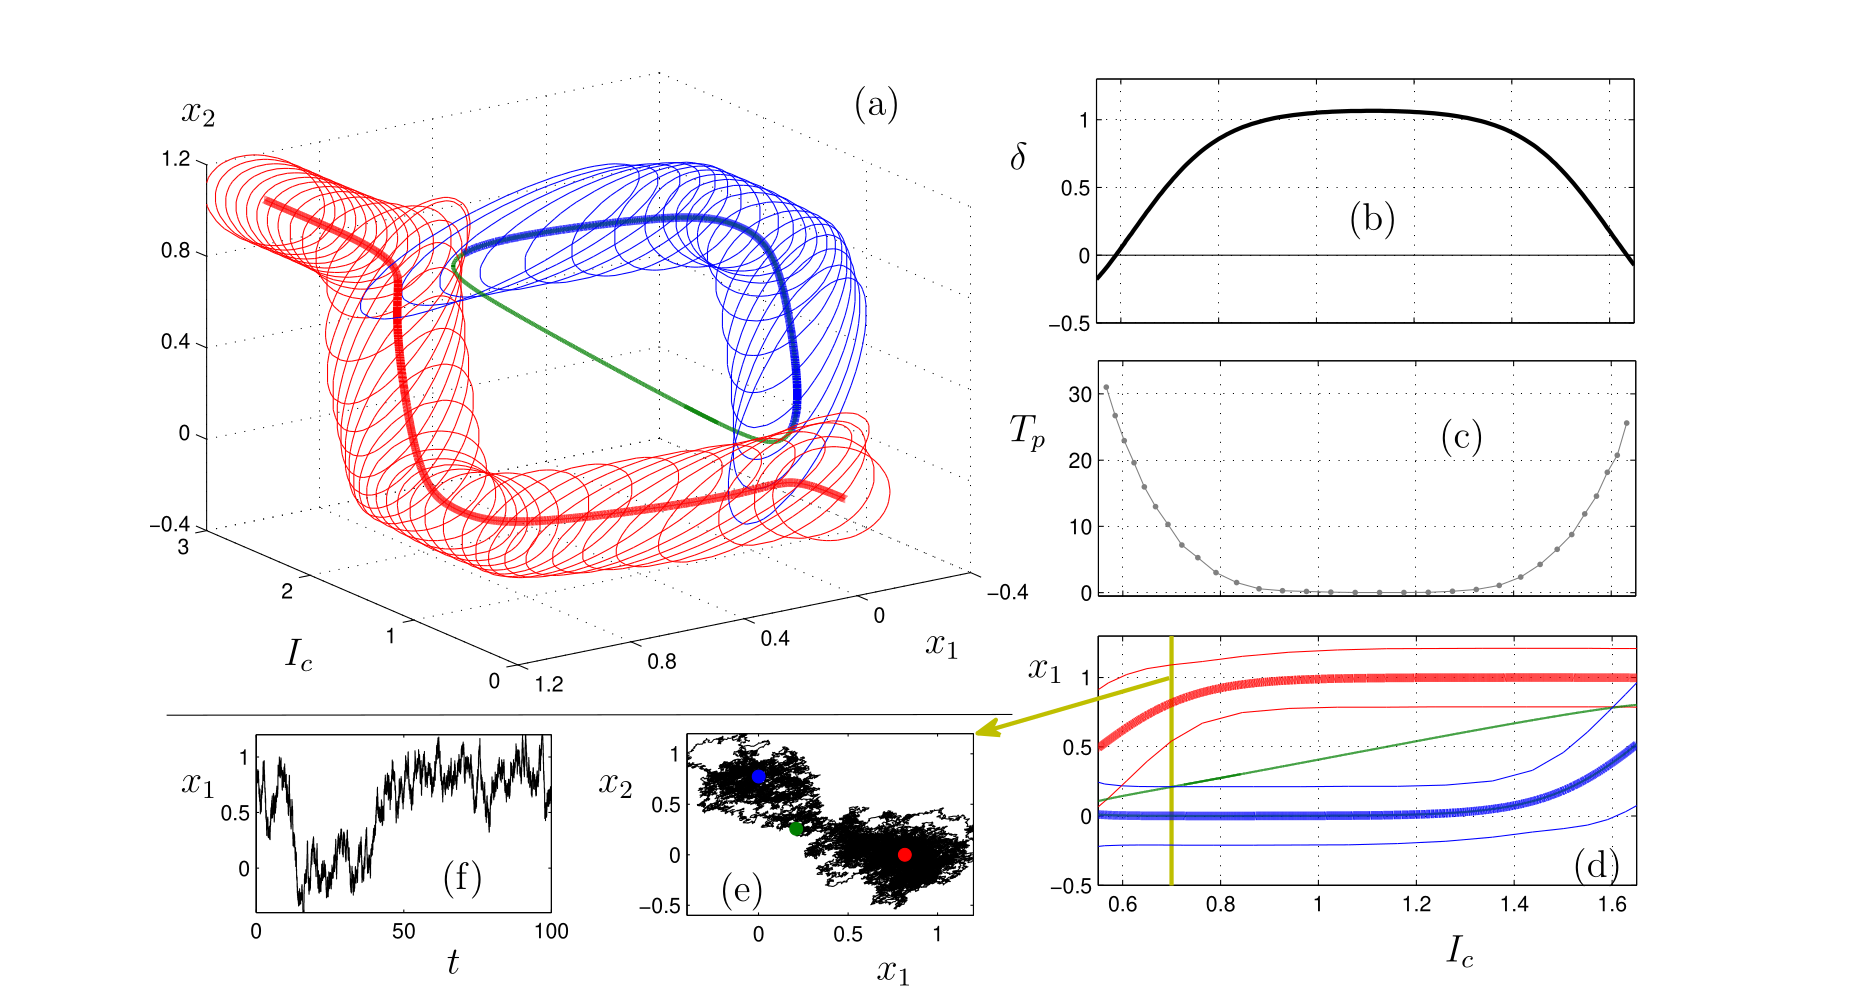
\includegraphics[width=.9\linewidth]{./example.png}
\end{center}
\end{frame}
\begin{frame}[label={sec:orgddca378}]{Example results}
\begin{center}
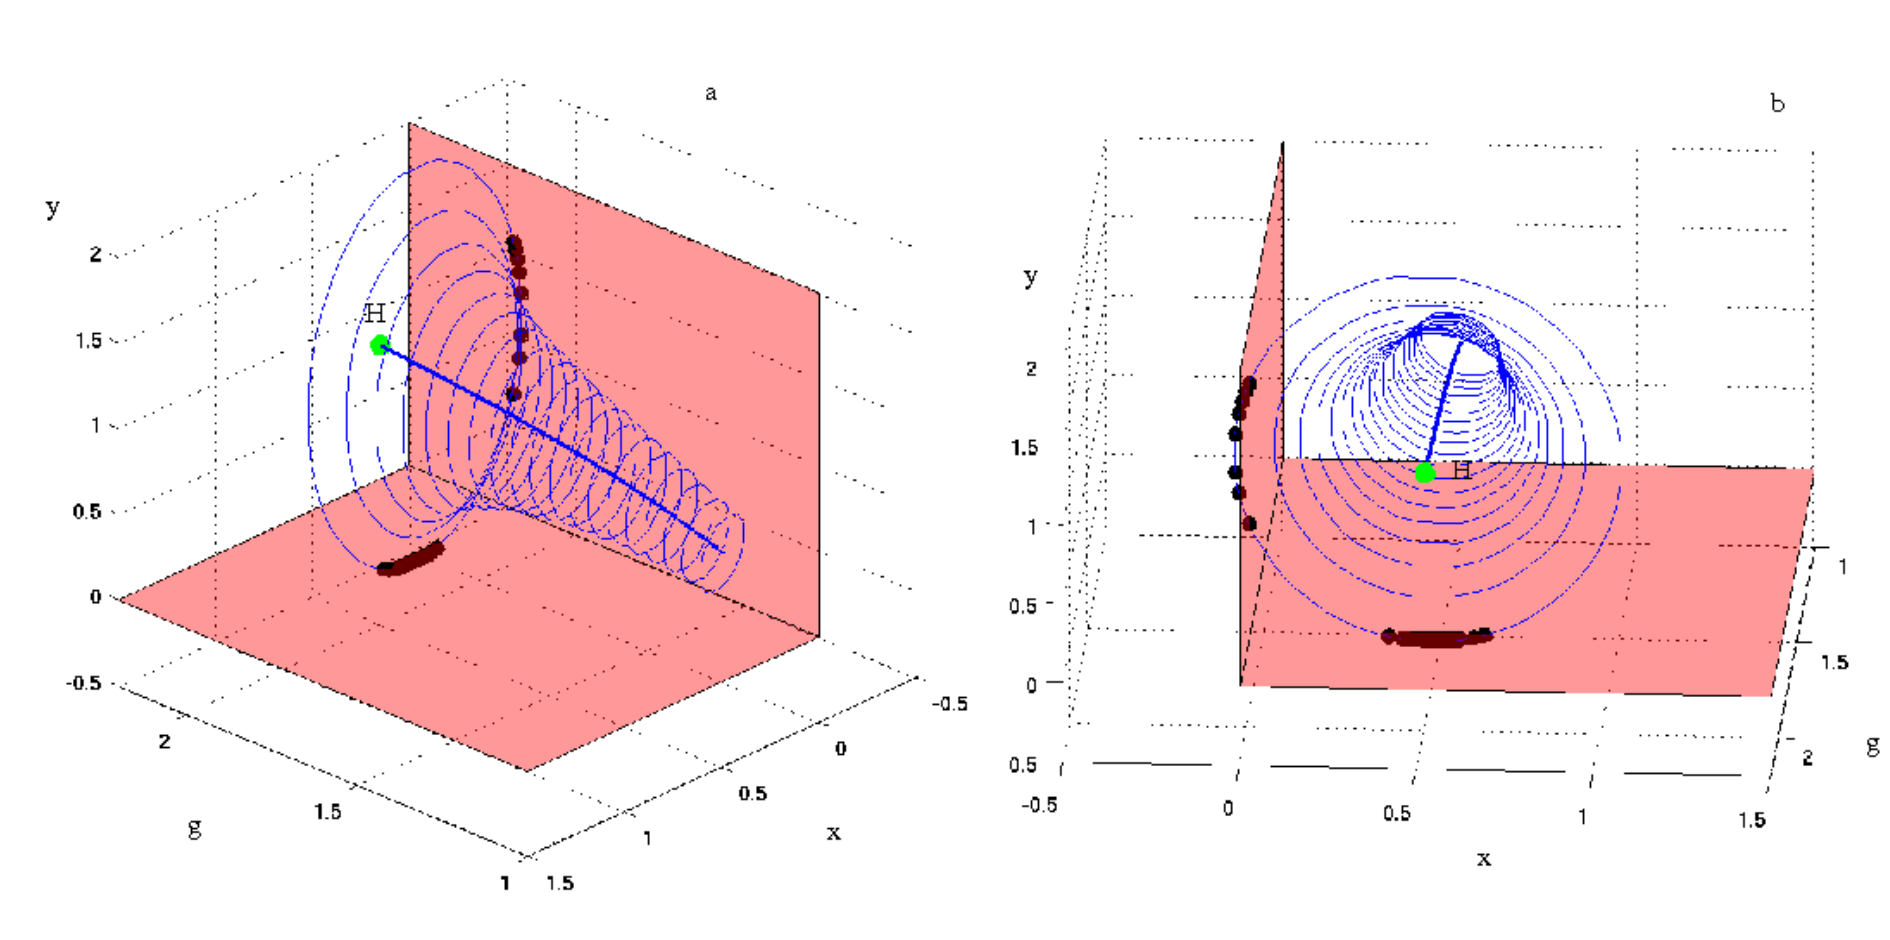
\includegraphics[width=.9\linewidth]{./hopf.png}
\end{center}
\end{frame}

\section{Section 9}
\label{sec:org56824c2}
\begin{frame}[label={sec:org0642513}]{Closing remark: a special case}
\begin{itemize}
\item Ellipsoid separation is only a local heuristic for stochastic timescales
\end{itemize}
\vfill
\begin{itemize}
\item What if we could incorporate global information into the continuation?
\end{itemize}
\vfill
\begin{itemize}
\item Eyring-Kramer's law gives analytical switching rates in special cases
\end{itemize}
\end{frame}
\end{document}
